\documentclass{beamer}
%
% Choose how your presentation looks.
%
% For more themes, color themes and font themes, see:
% http://deic.uab.es/~iblanes/beamer_gallery/index_by_theme.html
%
\mode<presentation>
{
  \usetheme{default}      % or try Darmstadt, Madrid, Warsaw, ...
  \usecolortheme{beaver} % or try albatross, beaver, crane, ...
  \usefonttheme{default}  % or try serif, structurebold, ...
  \setbeamertemplate{navigation symbols}{}
  \setbeamertemplate{caption}[numbered]
} 

\usepackage[english]{babel}
\usepackage[utf8x]{inputenc}
\usepackage{hyperref}
\hypersetup{
    colorlinks=true,
    linkcolor=blue,
    filecolor=magenta,      
    urlcolor=blue,
}

\title[Feedback \& Interactivity]{Feedback \& Interactivity}
\author{Andrés Pérez}
\institute{Digital Lutherie\\Master en Música para Experiencias del Entretenimiento\\ENTI-UB}
\date{2018/2019}

\newcommand\blfootnote[1]{%
  \begingroup
  \renewcommand\thefootnote{}\footnote{#1}%
  \addtocounter{footnote}{-1}%
  \endgroup
}

\AtBeginSection[]
{
\begin{frame}{Outline}
    \tableofcontents[currentsection] 
\end{frame}
}

\begin{document}

\begin{frame}
  \titlepage
\end{frame}



\begin{frame}{Outline}
 \tableofcontents
\end{frame}

%%%%%%%%%%%%%%%%%%%%%%%%%%%%%%%%%%%%%%%%%%%%%%%%%%
%%%%%%%%%%%%%%%%%%%%%%%%%%%%%%%%%%%%%%%%%%%%%%%%%%
%%%%%%%%%%%%%%%%%%%%%%%%%%%%%%%%%%%%%%%%%%%%%%%%%%
\section{Feedback}

\begin{frame}{Feedback}
    \begin{figure}[h]
        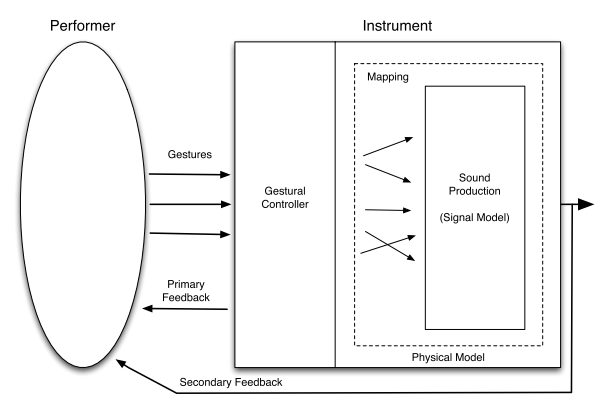
\includegraphics[width=0.9\textwidth]{instrument_scheme.png}\blfootnote{Wanderley, M. M. (2001). Performer-Instrument Interaction: Applications to Gestural Control of Sound Synthesis. PhD thesis, University Paris 6.}
    \end{figure}
\end{frame}

\begin{frame}{Feedback}
    (Tentative definition)\\
    \vspace{5mm}
    \textit{Feedback} is the information flow from the instrument to the performer.
\end{frame}

\begin{frame}{Feedback}
    Wanderley's Taxonomy\footnote{Wanderley, M. M. (2001). Gestural Control of Music. International Workshop Human Supervision and Control in Engineering and Music.}:\\
    \vspace{5mm}
    \begin{itemize}
        \item Primary Feedback
        \item Secondary Feedback
    \end{itemize}
\end{frame}

\begin{frame}{Feedback}
    \textbf{Primary Feedback}\\
    \vspace{5mm}
    Feedback produced by the input controller.
    \begin{itemize}
        \item Visual
        \item Tactile
        \item Acoustic
        \item Haptic
    \end{itemize}
\end{frame}

\begin{frame}{Feedback}
    \textbf{Secondary Feedback}\\
    \vspace{5mm}
    Acoustic output of the instrument's sound synthesis.
\end{frame}


\begin{frame}{Feedback}
    Feedback on acoustic instruments:\\
    \vspace{5mm}
    \textit{"[...] Studies of human performance have shown that while beginners generally rely on visual feedback, those who have mastered their instrument make use of haptic and tactile feedback."}\footnote{Marshall, M. T. (2008). Physical Interface Design for Digital Musical Instruments.}\\
    \vspace{5mm}
    \textit{"[...] We must stress that the relative importance of kinesthetic, tactile and visual feedback very much depends on the learning phase."}\footnote{Vertegaal, R., Ungvary, T., \& Kieslinger, M. (2000). Towards a Musician' s Cockpit : Transducers , Feedback and Musical Function.}
    
\end{frame}

\begin{frame}{Feedback}
    What about DMIs?\footnote{Marshall, M. T. (2008). Physical Interface Design for Digital Musical Instruments.}\\
    \begin{itemize}
        \item Bodyless instruments: no haptic/tactile feedback.
        \item Generally, no vibrotactile feedback from the interface due to secondary feedback.
        \item Generally, no secondary feedback from the interface location.
        \item Generally, small haptic feedback: lack of effort
    \end{itemize}
    AKA "\textit{the feel}" of the instrument...
\end{frame}

\begin{frame}{Feedback}
    Why is \textit{the feel} important?\\
\end{frame}

%%%%%%%%%%%%%%%%%%%%%%%%%%%%%%%%%%%%%%%%%%%%%%%%%%
%%%%%%%%%%%%%%%%%%%%%%%%%%%%%%%%%%%%%%%%%%%%%%%%%%
%%%%%%%%%%%%%%%%%%%%%%%%%%%%%%%%%%%%%%%%%%%%%%%%%%
\section{Interactivity}

%%%%%%%%%%%%%%%%%%%%%%%%%%%%%%%%%%%%%%%%%%%%%%%%%%
\subsection{Definition}

\begin{frame}{Interactivity - Definition} 
    What is \textit{interactivity?}
\end{frame}

\begin{frame}{Interactivity - Definition} 
    \textit{"Across the many fields concerned with interactivity, including information science, computer science, human-computer interaction, communication, and industrial design, there is little agreement over the meaning of the term 'interactivity'."}\footnote{Wikipedia. Interactivity. https://en.wikipedia.org/wiki/Interactivity. Accessed 19/02/2019}
\end{frame}

\begin{frame}{Interactivity - Definition} 
    \textit{"Interactivity is an expression of the extent that, in a given series of communication exchanges, any third (or later) transmission (or message) is related to the degree to which previous exchanges referred to even earlier transmissions."}\footnote{Rafaeli, S. (1988). From new media to communication. Sage annual review of communication research: Advancing communication science, 16, 110-134.}
\end{frame}

\begin{frame}{Interactivity - Definition} 
    \textit{"For full interactivity to occur, communication roles need to be interchangeable: role assignment and turn-taking are to be nonautomatic or nearly so".}\footnote{Rafaeli, S. (1988). From new media to communication. Sage annual review of communication research: Advancing communication science, 16, 110-134.}
\end{frame}

\begin{frame}{Interactivity - Definition} 
    \textit{"Interactivity varies along a continuum."}\footnote{Rafaeli, S., \& Sudweeks, F. (1997). Networked interactivity. Journal of computer-mediated communication, 2(4), JCMC243.}\\
    \vspace{5mm}
    Communication modes: \\
    Declarative $<---->$ Reactive  $<---->$ Interactive
\end{frame}

\begin{frame}{Interactivity - Definition} 
    \begin{figure}[h]
        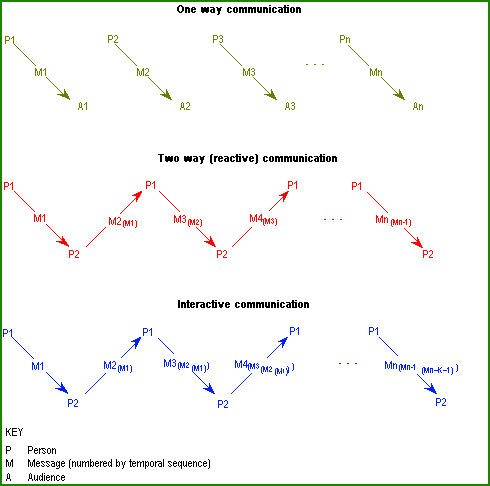
\includegraphics[width=0.65\textwidth]{interactivity_model.png} \blfootnote{Rafaeli, S., \& Sudweeks, F. (1997). Networked interactivity. Journal of computer-mediated communication, 2(4), JCMC243.}
    \end{figure}
\end{frame}

\begin{frame}{Interactivity - Definition} 
    \begin{figure}[h]
        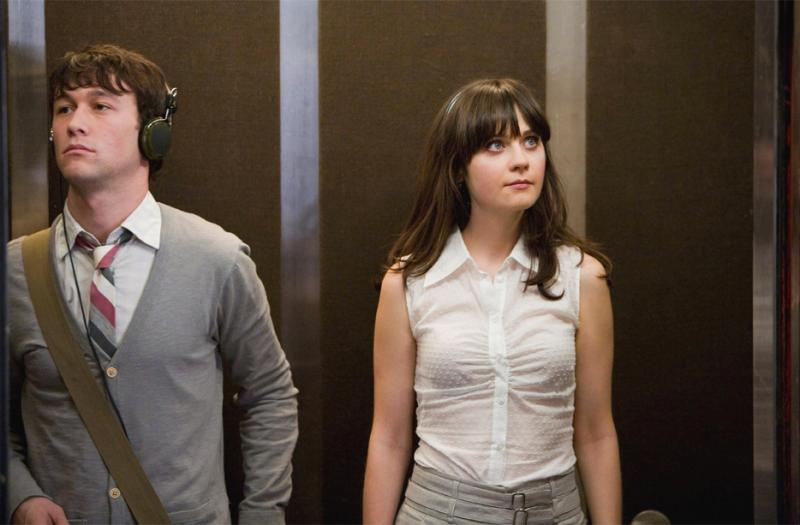
\includegraphics[width=\textwidth]{ascensor.jpg}
    \end{figure}
\end{frame}

\begin{frame}{Interactivity - Definition} 
    \begin{figure}[h]
        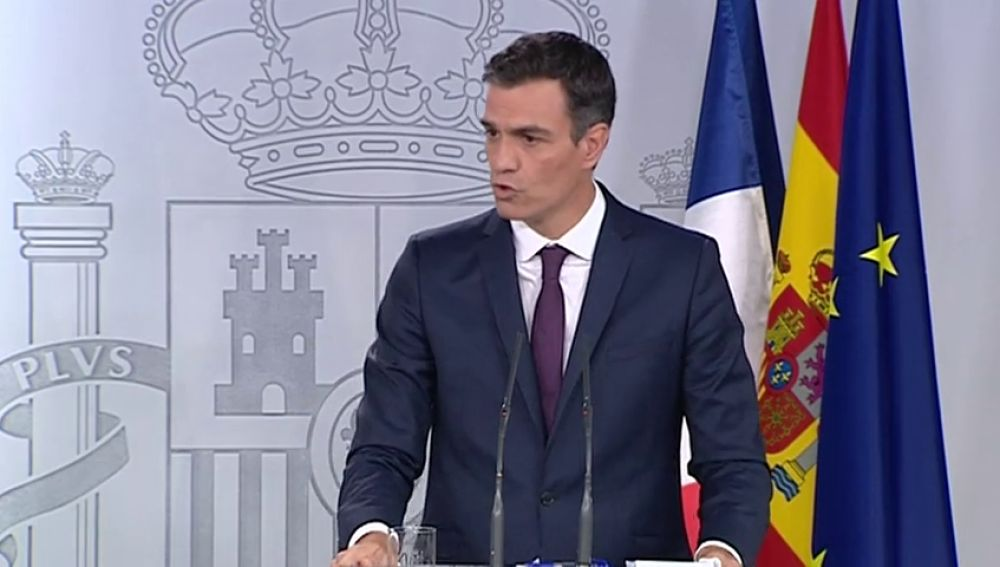
\includegraphics[width=\textwidth]{pedrosanchez.jpg}
    \end{figure}
\end{frame}

\begin{frame}{Interactivity - Definition} 
    \begin{figure}[h]
        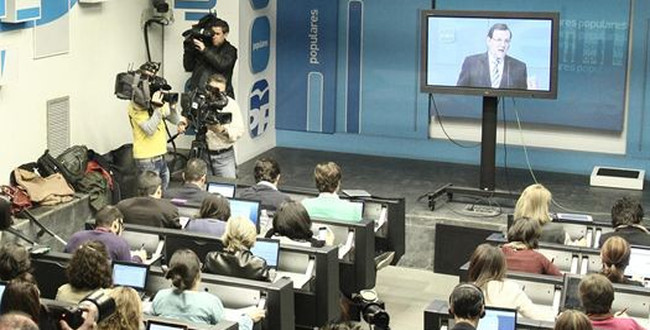
\includegraphics[width=\textwidth]{rajow.jpg}
    \end{figure}
\end{frame}

\begin{frame}{Interactivity - Definition} 
    \begin{figure}[h]
        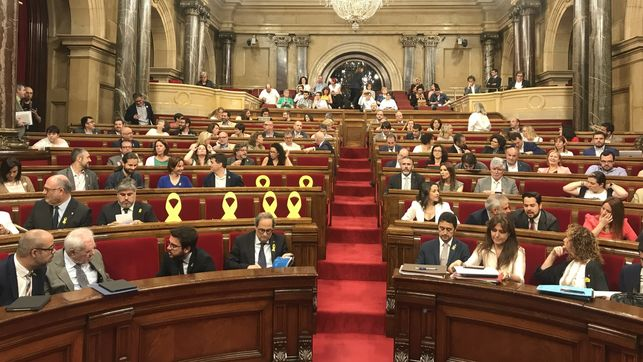
\includegraphics[width=\textwidth]{catalunya.jpg}
    \end{figure}
\end{frame}

\begin{frame}{Interactivity - Definition} 
    \begin{figure}[h]
        
\includegraphics[width=\textwidth]{bandersnatch.jpg}
    \end{figure}
\end{frame}


%%%%%%%%%%%%%%%%%%%%%%%%%%%%%%%%%%%%%%%%%%%%%%%%%%
\subsection{Human Computer Interaction}

\begin{frame}{Interactivity - HCI} 
   \textit{"\textbf{Human-Computer Interaction} (\textbf{HCI}) is a multidisciplinary field of study focusing on the design of computer technology and, in particular, the interaction between humans (the users) and computers."}\footnote{Interactive Design Foundation. What is HCI? https://www.interaction-design.org/literature/topics/human-computer-interaction. Accessed 19/02/2019}
\end{frame}

\begin{frame}{Interactivity - HCI} 
    \begin{figure}[h]
        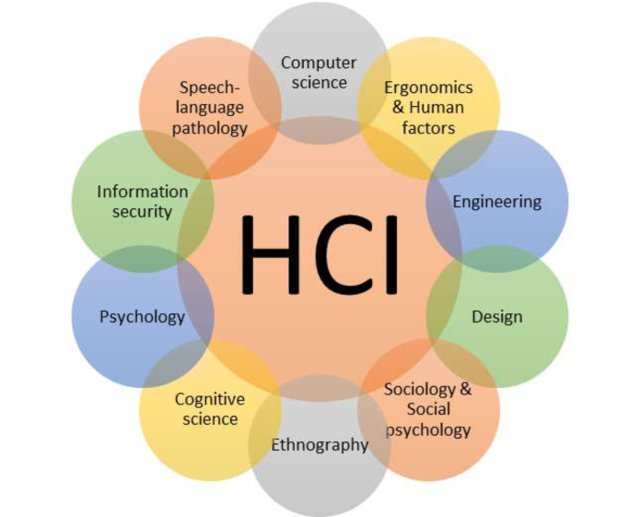
\includegraphics[width=0.85\textwidth]{hci.jpg}
    \end{figure}
\end{frame}

\begin{frame}{Interactivity - HCI} 
   \textit{"HCI concerns the design, evaluation, and implementation of interactive  computing  systems  for human  use  and  with  the  study  of  major  phenomena  surrounding them, especially in the context of the user’s task and work."}\footnote{Chakraborty, B. K., Sarma, D., Bhuyan, M. K., \& MacDorman, K. F. (2017). Review of constraints on vision-based gesture recognition for human–computer interaction. IET Computer Vision, 12(1), 3-15.}
\end{frame}

\begin{frame}{Interactivity - HCI} 
   \textit{"HCI concerns the \textbf{design}, \textbf{evaluation}, and \textbf{implementation} of interactive  computing  systems  for human  use  and  with  the  study  of  major  phenomena  surrounding them, especially \textbf{in the context of the user’s task} and work."}\footnote{Chakraborty, B. K., Sarma, D., Bhuyan, M. K., \& MacDorman, K. F. (2017). Review of constraints on vision-based gesture recognition for human–computer interaction. IET Computer Vision, 12(1), 3-15.}
\end{frame}

\begin{frame}{Interactivity - HCI} 
    HCI is built on top of \textit{Ergonomics}.\\
    \vspace{5mm}
    \textit{"\textbf{Ergonomics} (or \textbf{human factors}) is the scientific discipline concerned with the understanding of interactions among humans and other elements of a system, and the profession that applies theory, principles, data and methods to design in order to optimize human well-being and overall system performance."}\footnote{International Ergonomics Association. What is Ergonomics? https://www.iea.cc/whats/index.html. Accessed 19/02/2019.}
\end{frame}

\begin{frame}{Interactivity - HCI} 
    \begin{figure}[h]
        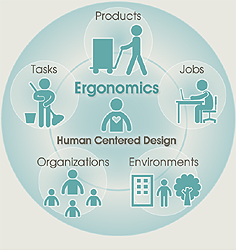
\includegraphics[width=0.6\textwidth]{ergonomics.png}
    \end{figure}\blfootnote{International Ergonomics Association. What is Ergonomics? https://www.iea.cc/whats/index.html. Accessed 19/02/2019.}
\end{frame}


\begin{frame}{Interactivity - HCI} 
    HCI Precursors
    \begin{figure}[h]
        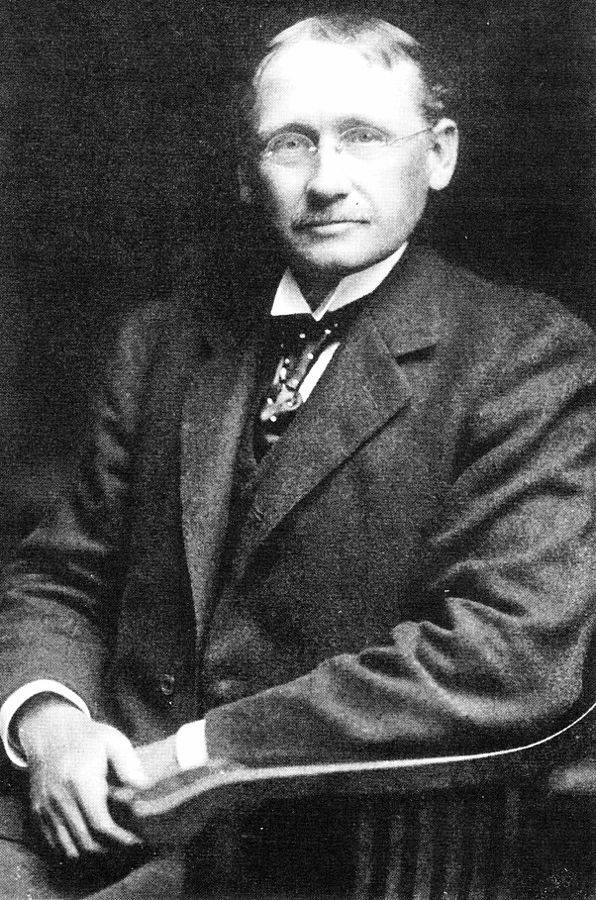
\includegraphics[width=0.4\textwidth]{taylor.jpg}
    \end{figure}
\end{frame}

\begin{frame}{Interactivity - HCI} 
    HCI Precursors\\
    \vspace{5mm}

    Frederick Winslow Taylor\\ 
    \begin{itemize}
        \item Scientific Management
        \item Application of rationality and empiricism to improve economic efficiency and productivity.\blfootnote{Wikipedia. Scientific Management. https://en.wikipedia.org/wiki/Scientific\_management}
    \end{itemize}
\end{frame}

\begin{frame}{Interactivity - HCI} 
    HCI Precursors
    \begin{figure}[h]
        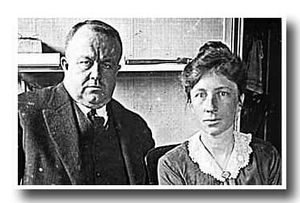
\includegraphics[width=0.8\textwidth]{gilbreth.jpg}
    \end{figure}
\end{frame}

\begin{frame}{Interactivity - HCI} 
    HCI Precursors\\
    \vspace{5mm}
    Frank \& Lilian Gilbreth\\ 
    \begin{itemize}
        \item Time and motion study
        \item \textit{"[...] They aimed to improve efficiency by eliminating unnecessary steps and actions. By applying this approach, the Gilbreths reduced the number of motions in bricklaying from 18 to 4.5, allowing bricklayers to increase their productivity from 120 to 350 bricks per hour."}\blfootnote{Wikipedia. Human Factors and Ergonomics. https://en.wikipedia.org/wiki/Human\_factors\_and\_ergonomics}
    \end{itemize}
\end{frame}

\begin{frame}{Interactivity - HCI} 
    HCI Precursors
    \begin{figure}[h]
        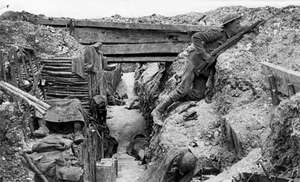
\includegraphics[width=\textwidth]{ww1.jpg}
    \end{figure}
\end{frame}

\begin{frame}{Interactivity - HCI} 
    HCI Precursors\\
    \vspace{5mm}
    World War I\\ 
    \begin{itemize}
        \item Studies on pilot success: aircraft design, simulators
        \item Ford: Studies on driver behavior
    \end{itemize}
\end{frame}

\begin{frame}{Interactivity - HCI} 
    HCI Precursors
    \begin{figure}[h]
        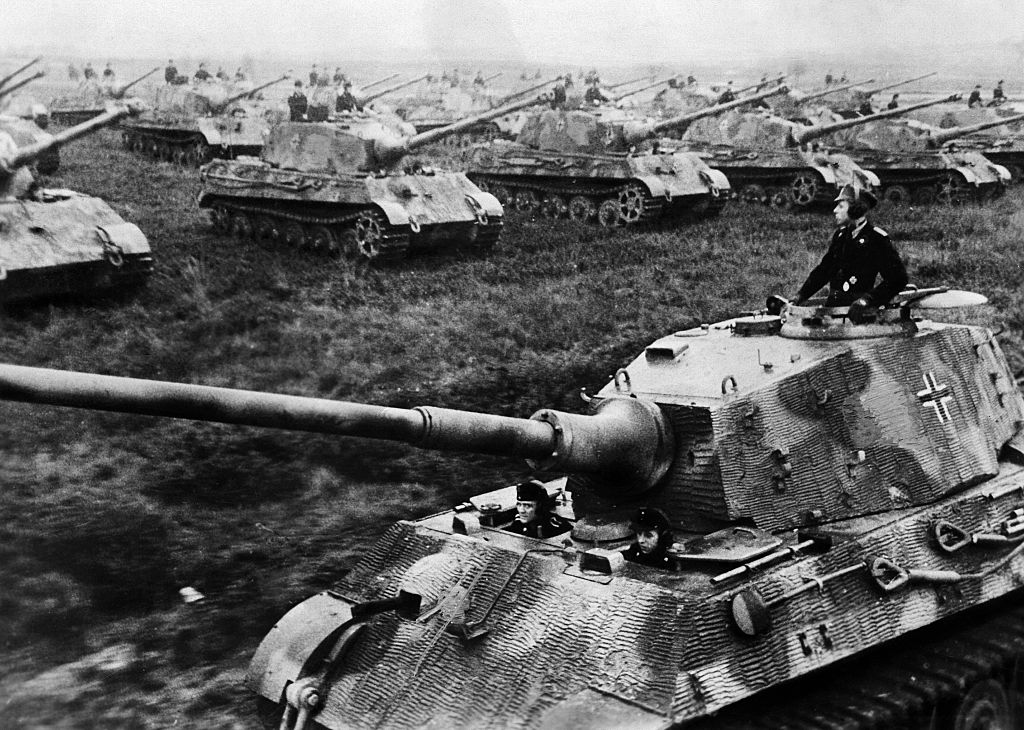
\includegraphics[width=0.9\textwidth]{ww2.jpg}
    \end{figure}
\end{frame}

\begin{frame}{Interactivity - HCI} 
    HCI Precursors\\
    \vspace{5mm}
    World War II\\ 
    \begin{itemize}
        \item Studies on operator cognition
        \item Alphonse Chapanis: aircraft control's \textit{shape coding}
        \item Paul Fitts: \textit{Fitts' Law}
    \end{itemize}
\end{frame}

\begin{frame}{Interactivity - HCI} 
    HCI Precursors\\
    Shape Coding
    \begin{figure}[h]
        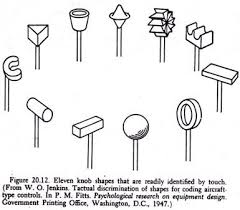
\includegraphics[width=0.7\textwidth]{shapecoding.jpeg}
    \end{figure}
\end{frame}

\begin{frame}{Interactivity - HCI} 
    HCI Precursors\\
    Fitt's Law
    \begin{figure}[h]
        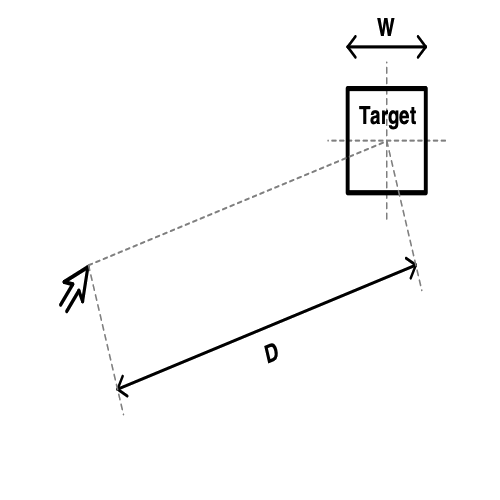
\includegraphics[width=0.5\textwidth]{fittslaw.png}\blfootnote{By Foobar628 - Own work, CC BY-SA 4.0, https://commons.wikimedia.org/w/index.php?curid=69865276}
    \end{figure}
\end{frame}

\begin{frame}{Interactivity - HCI} 
    HCI Precursors\\
    Fitt's Law\\
    \vspace{5mm}
    Index of Difficulty:
    \begin{equation*}
        ID = log_2\frac{2D}{W}
    \end{equation*}
    Index of Performance (\textit{Throughput}):
    \begin{equation*}
        IP = \frac{ID}{MT}
    \end{equation*}
\end{frame}

\begin{frame}{Interactivity - HCI} 
    HCI Precursors\\
    \vspace{5mm}
    Xerox Experiment (1978)\footnote{Card, Stuart K.; English, William K.; Burr, Betty J. (1978). "Evaluation of mouse, rate-controlled isometric joystick, step keys, and text keys for text selection on a CRT". Ergonomics. 21 (8): 601–613.}\\ 
    \begin{itemize}
        \item First application of Fitts' Law on HCI
        \item Commercial introduction of mouse for PCs
    \end{itemize}
\end{frame}

\begin{frame}{Interactivity - HCI} 
    HCI Precursors\\
    Xerox Experiment
    \begin{figure}[h]
        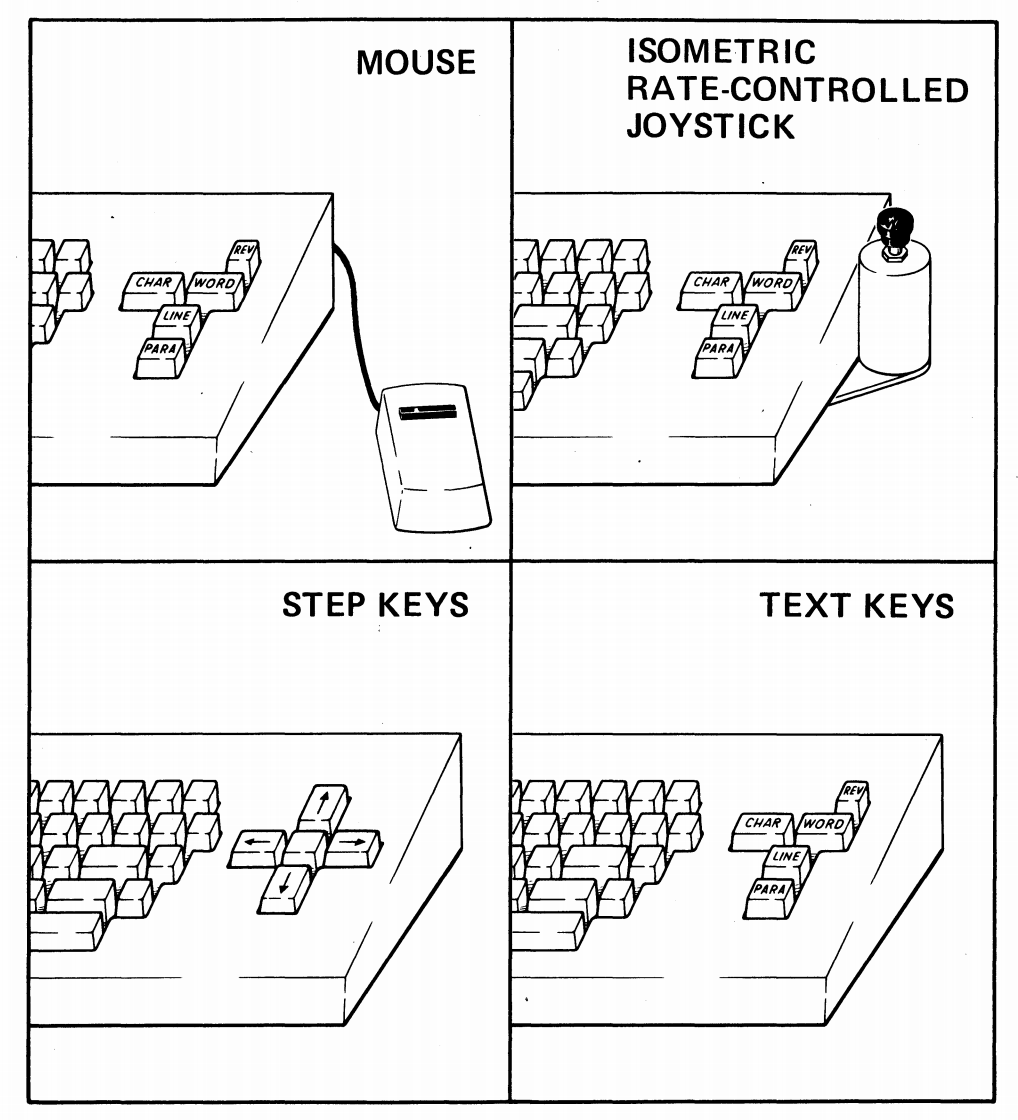
\includegraphics[width=0.6\textwidth]{xerox2.png}
    \end{figure}
\end{frame}

\begin{frame}{Interactivity - HCI} 
    HCI Precursors\\
    Xerox Experiment
    \begin{figure}[h]
        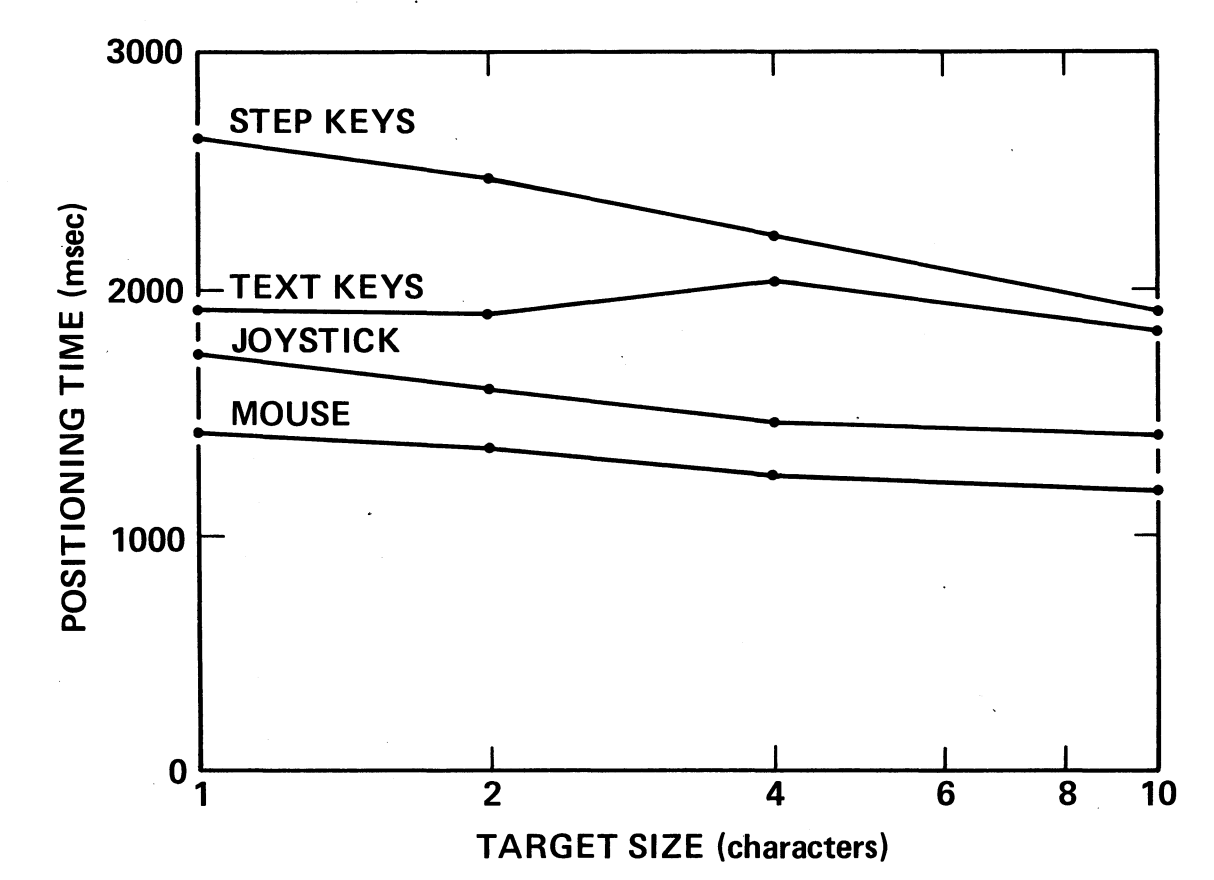
\includegraphics[width=0.8\textwidth]{xerox.png}
    \end{figure}
\end{frame}

\begin{frame}{Interactivity - HCI} 
    HCI Precursors\\
    \vspace{5mm}
    Interaction Design Principles: Machintosh vs Windows:\footnote{Tognazzinim B.  "First Principles of Interaction Design".https://asktog.com/atc/principles-of-interaction-design/}\\ 
    \begin{itemize}
        \item \textit{"Fitts’s law [...] dictates the Macintosh pull-down menu acquisition should be approximately five times faster than Windows menu acquisition, and this is proven out."}
        \item \textit{"Fitts’s law predicted that the Windows Start menu was built upside down, with the most used applications farthest from the entry point, and tests proved that out."} 
        \item \href{https://www.quora.com/Does-fitts-law-work-differently-in-Mac-and-Windows}{Quora: Does fitts law work differently in Mac and Windows?}
    \end{itemize}
\end{frame}


%%%%%%%%%%%%%%%%%%%%%%%%%%%%%%%%%%%%%%%%%%%%%%%%%%
\subsection{DMI Interaction}

\begin{frame}{Interactivity - DMI Interaction} 
    Early attempts: apply HCI analysis to musical tasks\\
\end{frame}

\begin{frame}{Interactivity - DMI Interaction} 
    Hunt's experiment (2000)\footnote{Hunt, A. (2000). Mapping Strategies for Musical Performance.}: compare the performance of different interfaces/mappings for a given task.
\end{frame}

\begin{frame}{Interactivity - DMI Interaction} 
    Hunt's experiment\\
    \vspace{5mm}
    Interfaces:
    \begin{itemize}
        \item Mouse
        \item Sliders
        \item Multiparametric (no visual feedback)
    \end{itemize}
    Synth parameters:
    \begin{itemize}
        \item Volume
        \item Pitch
        \item Timbre
        \item Panning
    \end{itemize}
\end{frame}

\begin{frame}{Interactivity - DMI Interaction} 
    Hunt's experiment\\
    \vspace{5mm}
    \begin{figure}[h]
        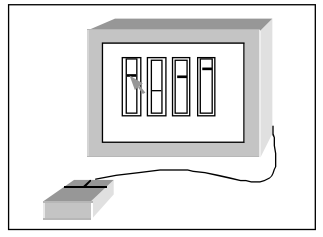
\includegraphics[width=0.5\textwidth]{Hunt2000_interfaceA.png}
        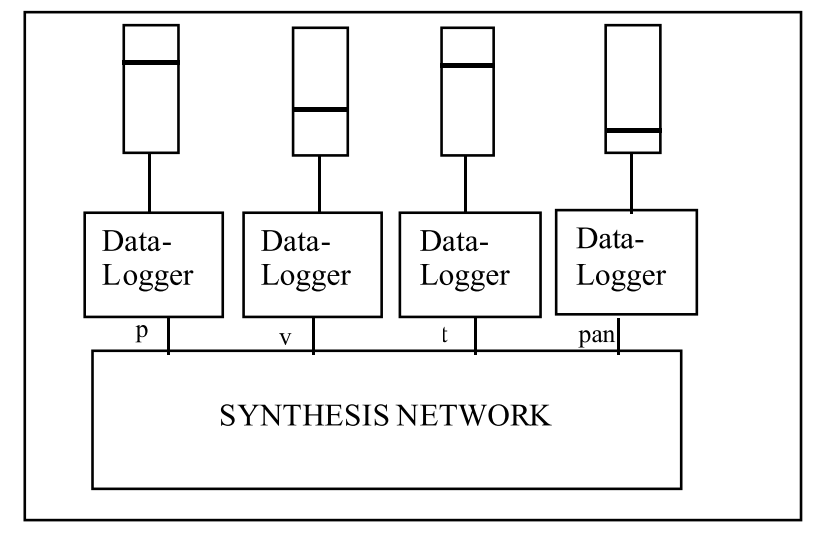
\includegraphics[width=0.5\textwidth]{hunt2000_mapping_a.png}
    \end{figure}
\end{frame}

\begin{frame}{Interactivity - DMI Interaction} 
    Hunt's experiment\\
    \vspace{5mm}
    \vspace{5mm}
    \begin{figure}[h]
        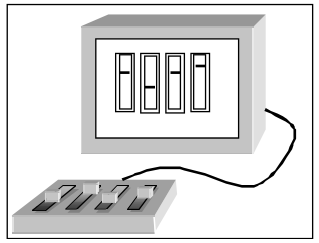
\includegraphics[width=0.5\textwidth]{hunt2000_interfaceB.png}
        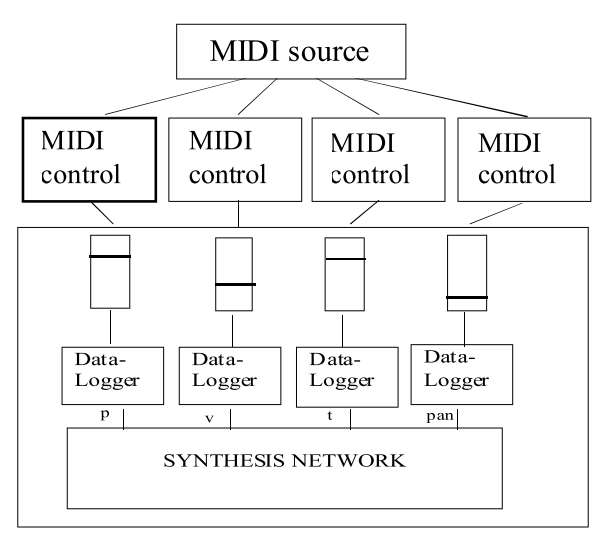
\includegraphics[width=0.5\textwidth]{hunt2000_mapping_b.png}
    \end{figure}
\end{frame}

\begin{frame}{Interactivity - DMI Interaction} 
    Hunt's experiment\\
    \vspace{5mm}
    \begin{figure}[h]
        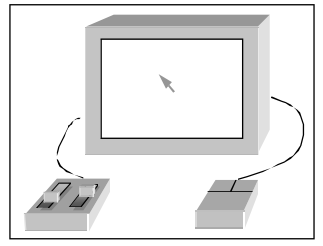
\includegraphics[width=0.5\textwidth]{hunt2000_interfaceC.png}
        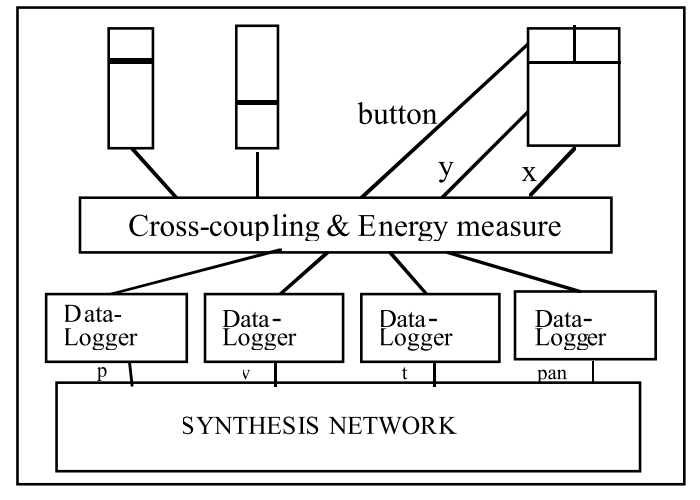
\includegraphics[width=0.5\textwidth]{hunt2000_mapping_c.png}
    \end{figure}
\end{frame}

\begin{frame}{Interactivity - DMI Interaction} 
    Hunt's experiment\\
    \vspace{5mm}
    Multiparametric interface mapping:
    \begin{itemize}
        \item Volume = speed of mouse + mouse button pressed + average position of two sliders.
        \item Pitch = vertical position of the mouse + speed of movement of slider no. 2.
        \item Timbre = Horizontal position of the mouse + difference in the two slider positions. 
        \item Panning = Position of slider no. 1.
    \end{itemize}
\end{frame}

\begin{frame}{Interactivity - DMI Interaction} 
    Hunt's experiment\\
    \vspace{5mm}
    \begin{figure}[h]
        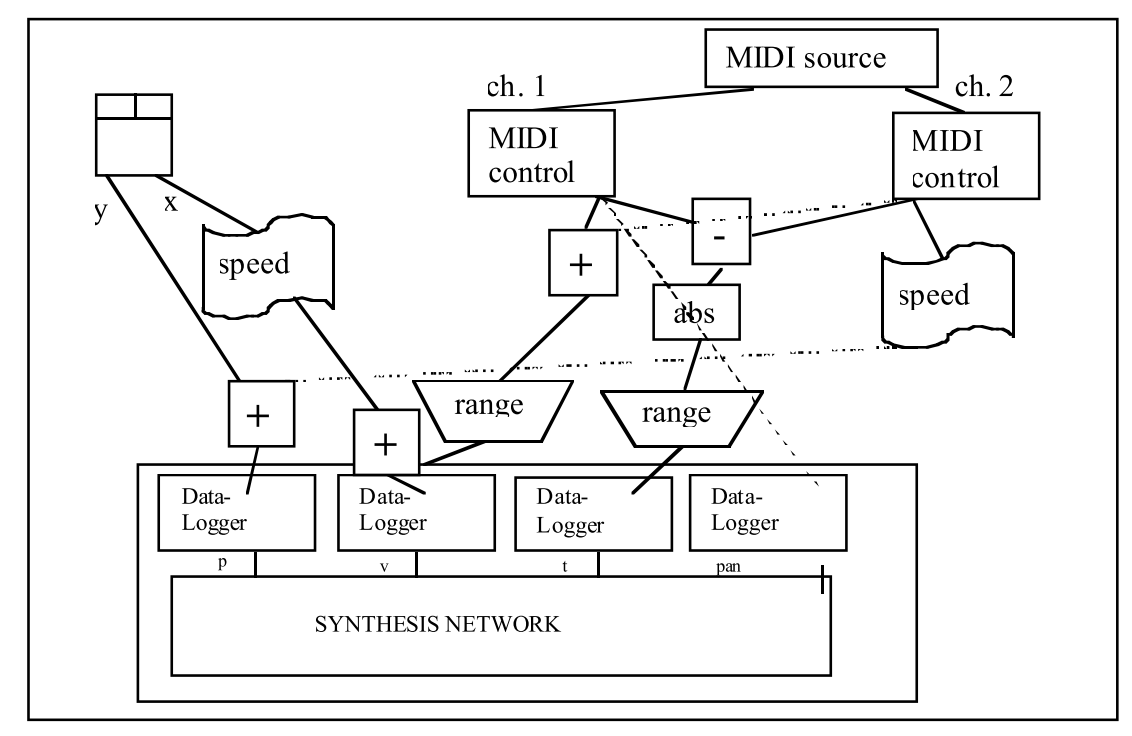
\includegraphics[width=0.9\textwidth]{hunt2000_mapping_c2.png}
    \end{figure}
\end{frame}


\begin{frame}{Interactivity - DMI Interaction} 
    Hunt's experiment\\
    \vspace{5mm}
    Task:
    \begin{itemize}
        \item Accurately replicate a given sound
        \item 2-4 seconds long
        \item 3 difficulty groups, 24 sounds per group
        \item 3 different sessions, 45 minutes per session
    \end{itemize}
\end{frame}

\begin{frame}{Interactivity - DMI Interaction} 
    Hunt's experiment\\
    \vspace{5mm}
    Evaluation:
    \begin{itemize}
        \item Timing
        \item Parameter
        \item Trajectory
    \end{itemize}
    ... all evaluated by the same human judge! (3456 tests)
\end{frame}

\begin{frame}{Interactivity - DMI Interaction} 
    Hunt's experiment\\
    \vspace{5mm}
    \begin{figure}[h]
        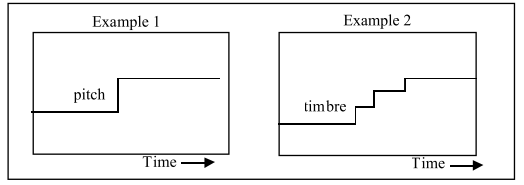
\includegraphics[width=\textwidth]{hunt2000_groupA.png}
    \end{figure}
\end{frame}

\begin{frame}{Interactivity - DMI Interaction} 
    Hunt's experiment\\
    \vspace{5mm}
    \begin{figure}[h]
        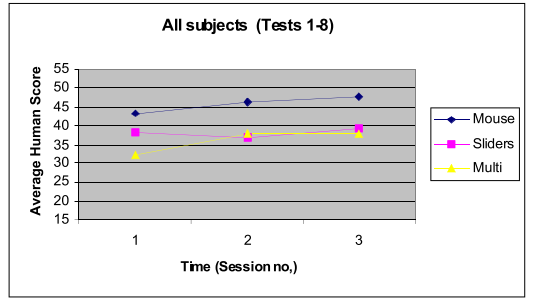
\includegraphics[width=\textwidth]{hunt2000_result1.png}
    \end{figure}
\end{frame}

\begin{frame}{Interactivity - DMI Interaction} 
    Hunt's experiment\\
    \vspace{5mm}
    \begin{figure}[h]
        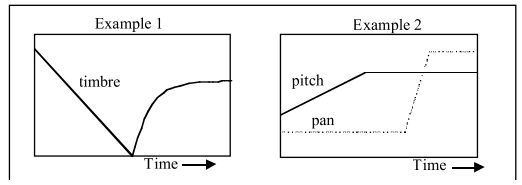
\includegraphics[width=\textwidth]{hunt2000_groupB.png}
    \end{figure}
\end{frame}

\begin{frame}{Interactivity - DMI Interaction} 
    Hunt's experiment\\
    \vspace{5mm}
    \begin{figure}[h]
        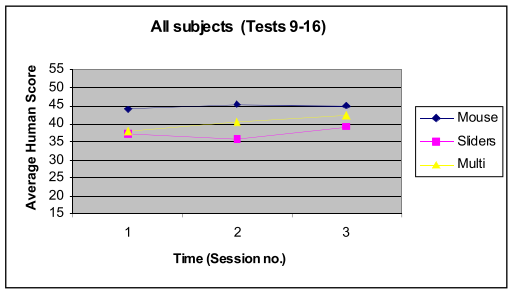
\includegraphics[width=\textwidth]{hunt2000_result2.png}
    \end{figure}
\end{frame}

\begin{frame}{Interactivity - DMI Interaction} 
    Hunt's experiment\\
    \vspace{5mm}
    \begin{figure}[h]
        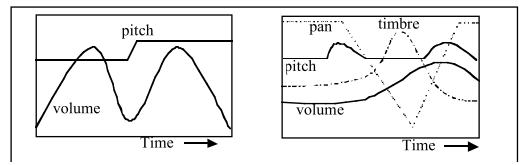
\includegraphics[width=\textwidth]{hunt2000_groupC.png}
    \end{figure}
\end{frame}

\begin{frame}{Interactivity - DMI Interaction} 
    Hunt's experiment\\
    \vspace{5mm}
    \begin{figure}[h]
        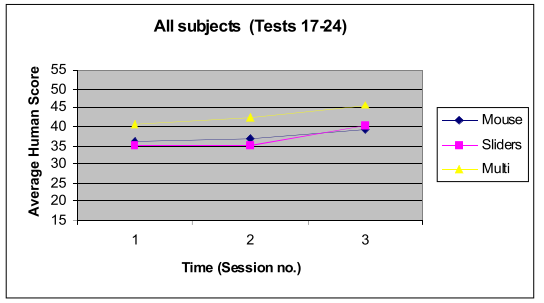
\includegraphics[width=\textwidth]{hunt2000_result3.png}
    \end{figure}
\end{frame}

\begin{frame}{Interactivity - DMI Interaction} 
    Hunt's experiment\\
    \vspace{5mm}
    \begin{figure}[h]
        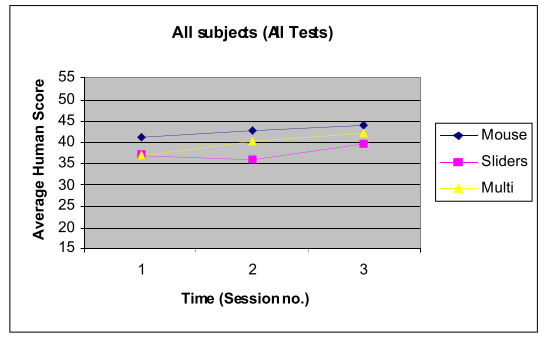
\includegraphics[width=\textwidth]{hunt2000_result4.png}
    \end{figure}
\end{frame}

\begin{frame}{Interactivity - DMI Interaction} 
    Hunt's experiment\\
    \vspace{5mm}
    Major conclusions:
    \begin{itemize}
        \item Real-time control can be enhanced by the multiparametric interface
        \item Mappings which are not one-to-one are more \textit{engaging} for users
        \item Complex tasks may need complex interfaces
        \item The mouse interface is good for simple tests and for little practice time
        \item Some people prefer to think in terms of separate parameters
    \end{itemize}
\end{frame}

\begin{frame}{Interactivity - DMI Interaction} 
    Hunt's experiment\\
    \vspace{5mm}
    Some subject's comments on the multiparametric instrument:
    \begin{itemize}
        \item \textit{"This feels multi-dimensional, gestural. I sometimes found myself thinking of a shape".}
        \item \textit{"I'm not thinking of timbre as a 'parameter' like I do with the sliders [...]} 
        \item \textit{"I could concentrate on the performance \textbf{without worrying} about the actual mechanics of it."}
        \item \textit{"You can use your \textbf{unconscious} to play it after a while. You can \textbf{forget} about the interface so that you can concentrate on the sound"}.
     \end{itemize}
\end{frame}
       
\begin{frame}{Interactivity - DMI Interaction} 
    Hunt's experiment\\
    \vspace{5mm}
    Some subject's comments on the multiparametric instrument:
    \begin{itemize}
        \item \textit{"It became more like driving a car - in that you've got physical actions that you can sort of get on with, leaving you free to think of other things".}
        \item \textit{"This is a lot \textbf{better} [...] even though I felt out of control".}
        \item \textit{"This is \textbf{really good fun}! Even when you're not doing so well!"}
        \item \textit{"One movement controlling several things is more fun. \textbf{It's not like a task} - it's \textbf{like playing an instrument}".}
        \item \textit{"This is intuitively \textbf{easier}"}
    \end{itemize}
\end{frame}

\begin{frame}{Interactivity - DMI Interaction} 
    Hunt's experiment\\
    \vspace{5mm}
    Some subject's comments on the multiparametric instrument:
    \begin{itemize}
        \item \textit{"This interface has \textbf{possibilities}. I'd choose this over the long term".}
        \item \textit{"I like this the best; definitely! It's a lot \textbf{freer} - more \textbf{flowing}".}
        \item \textit{"It's the easiest of the three. It has the \textbf{musical 'edge'}".}
        \item \textit{"This is the best interface. You've got more \textbf{freedom}, and there's so much \textbf{potential} if I could just get the hang of it".}
    \end{itemize}
\end{frame}



\begin{frame}{Interactivity - DMI Interaction} 
    \Large
    What does it mean \textit{"task"} in a musical context?
\end{frame}

\begin{frame}{Interactivity - DMI Interaction} 
    Some words appearing in Hunt's experiment:
    \begin{itemize}
        \item Not like a task
        \item Possibilities
        \item Freedom
        \item Potential
        \item Easy
        \item Flowing
        \item Musical edge
        \item Without worrying
        \item Unconscious
        \item Better
    \end{itemize}
\end{frame}

\begin{frame}{Interactivity - DMI Interaction} 
\textit{"The attributes of an instrumental real-time control system seem to be:}\blfootnote{Hunt, A. (2000). Mapping Strategies for Musical Performance.}
\begin{itemize}
    \item \textit{There is no fixed ordering to the human-computer \textbf{dialogue}.}
    \item \textit{The human takes control of the situation. The computer is reactive.}
    \item \textit{There is no single permitted set of options (e.g. choices from a menu) but rather a series of continuous controls.}
    \item \textit{There is an instant response to the user's movement}s.
    \item \textit{Similar movements produce similar results.}
\end{itemize}
...
\end{frame}

\begin{frame}{Interactivity - DMI Interaction} 
...
\begin{itemize}
    \item \textit{The overall control of the system (under the direction of the human operator) is the main goal, rather than the ordered transfer of information.}
    \item \textit{The control mechanism is a physical and multi-parametric device which must be learnt by the user until the actions become automatic.}
    \item \textit{Further practice develops increased control intimacy and thus competence of operation.}
    \item \textit{The human operator, once familiar with the system, is free to perform other cognitive activities whilst operating the system (e.g. talking while driving a car)."}\blfootnote{Hunt, A. (2000). Mapping Strategies for Musical Performance.}
\end{itemize}
\end{frame}


\begin{frame}{Interactivity - DMI Interaction} 
    The Zone\\
    \vspace{5mm}
    \textit{"In positive psychology, a \textbf{flow state}, also known colloquially as \textbf{being in the zone}, is the mental state of operation in which a person performing an activity is fully immersed in a feeling of energized focus, full involvement, and enjoyment in the process of the activity."}\footnote{Wikipedia. Flow (psychology). https://en.wikipedia.org/wiki/Flow\_(psychology). Accessed 19/02/2019.}
\end{frame}

\begin{frame}{Interactivity - DMI Interaction} 
    Nakamura \& Csíkszentmihályi\footnote{Nakamura, J.; Csikszentmihályi, M. (20 December 2001). "Flow Theory and Research". In C. R. Snyder Erik Wright, and Shane J. Lopez. Handbook of Positive Psychology.}:
    \begin{itemize}
        \item Intense and focused concentration on the present moment
        \item Merging of action and awareness
        \item A loss of reflective self-consciousness
        \item A sense of personal control or agency over the situation or activity
        \item A distortion of temporal experience
        \item Experience of the activity as intrinsically rewarding
    \end{itemize}
\end{frame}

\begin{frame}{Interactivity - DMI Interaction} 
    Additions by Cherry\footnote{Cherry, Kendra. "What is Flow?". About Education. Retrieved 30 March 2015}:
    \begin{itemize}
        \item \textbf{Immediate feedback}
        \item Feeling that you have the potential to succeed
        \item Feeling so engrossed in the experience, that other needs become negligible
    \end{itemize}
\end{frame}

\begin{frame}{Interactivity - DMI Interaction} 
    Csíkszentmihályi's Flow modes
    \begin{figure}[h]
        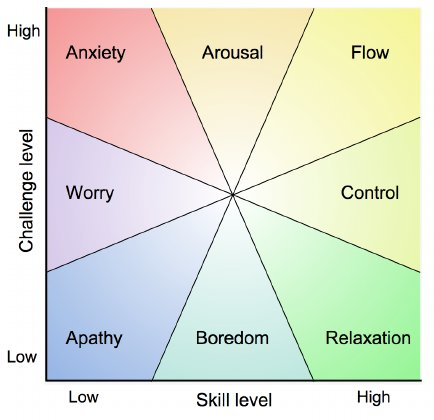
\includegraphics[width=0.65\textwidth]{flow.jpg}\blfootnote{Csikszentmihalyi, M., Finding Flow, 1997.}
    \end{figure}
\end{frame}


\begin{frame}{Interactivity - DMI Interaction} 
    \textit{"Most people who are employed to design user interfaces are highly analytical. They read the HCI literature which is highly analytical. They produce interfaces which suit highly analytical people. They represent only a small proportion of the population. Their interfaces are used by the population at large, the majority of which think in a very different way, and therefore find the interfaces difficult to use."}\footnote{Hunt, A. (2000). Mapping Strategies for Musical Performance.}
\end{frame}

\begin{frame}{Interactivity - DMI Interaction} 
    \textit{“A distinguishing feature of the musical context of gesture is that the human performer uses a combination of extensive training, anticipations of musical structure, and sensory feedback to continuously adjust and refine the gesture. Therefore, musical gestures cannot be directly compared to reaction-time studies or task-based assessments as they are used in the study of human-machine ergonomics.”}\footnote{Schmeder, A., Freed, A.,\& Wessel, D. (2010). Best Practices for Open Sound Control. Linux Audio Conference}
\end{frame}





\begin{frame}{Interactivity - DMI Interaction} 
    \textit{"Music, on the other hand, has always been a highly interactive activity. Musicians interact with their instrument,with other musicians,with dancers or with the audience [...] Recorded music eliminated the feedback dialogue between the audience and the live musicians, turning music performance into a one-way communication. Later, as a result of multitrack recording, even the dialogue between different players was eliminated."}\footnote{Jordà, S. (2007). Interactivity and live computer music. Computer Music Journal.}
\end{frame}








\end{document}
